\documentclass[12pt]{article}
\usepackage[utf8]{inputenc}
\usepackage[russian]{babel}
\usepackage[margin=1.5in,left=1cm,right=1cm, top=2cm,bottom=2cm,bindingoffset=0cm]{geometry}
\usepackage{graphicx}
\usepackage{color}
\usepackage{amssymb}
\usepackage{minted}
\usepackage{hyperref}
\usepackage{amsmath}
\usepackage{fancyhdr}



\title{Title}
\author{Амеличев Константин, ПМИ 191.}
\date{Date}

\newcommand{\problem}[2]{

\section {Задача #1}
\textbf {Постановка задачи.} {#2}

\textbf {Решение.}
}

\newcommand{\limit}[2]{\displaystyle \lim_{#1 \to #2}}

\newcommand{\rangesum}[2]{\displaystyle \sum_{#1}^{#2}}

\newcommand{\mintedparams}{
% frame=lines
% framesep=2mm,
% baselinestretch=1.2,
% bgcolor=LightGray    
}

\pagestyle{fancy}
\fancyhf{}
\fancyhead[LE,RO]{Амеличев Константин, ПМИ 191, @kik0s, \href{http://github.com/kik0s}{\textcolor{blue}{github}}, \href{http://codeforces.com/profile/kikos}{\textcolor{blue}{codeforces}}, \href{http://vk.com/i_tried_to_name_myself_kikos}{\textcolor{blue}{vk}}}
\fancyhead[RE,LO]{Лекция АиСД 14.01}

\begin{document}

\paragraph{Задачи на отрезке.} Введем какую-то произвольную операцию $\oplus$, и будем отвечать на запросы $get(l,\,r)$ на массиве $a$, ответом на которые будет $a_l \oplus a_{l+1} \oplus \dots \oplus a_r$. Также введем операцию изменения на отрезке $a_i := change(a_i,\,x)$.

Потребуем от $\oplus$ ассоциативность ~--- $a \oplus (b \oplus c) = (a \oplus b) \oplus c$.

\paragraph{Префиксные суммы.} Если в задаче нет запросов изменения (и элементы образуют группу, то есть есть обратный элемент), то посчитаем $p_i = p_{i-1} \oplus a_i$. Тогда ответ на запрос~--- это $p_r \oplus p_{l-1}^{-1}$. Если операция некоммутативна, то нужно будет пострадать, но вроде бы можно просто сделать $p_{l-1}^{-1} \oplus p_r$. Построение за $O(n)$, запрос за $O(1)$.

\paragraph{Sparse table.} Если элементы не образуют группу, но задача все еще статическая, то можно сохранить значения, соответствующие $\oplus$ по всем отрезкам длины $2^k$. Тогда, когда нужно ответить на запрос $get(l,\,r)$, можно взять перекрывающиеся отрезки $[l,\,l + 2^i)$ и $(r - 2^i,\,r]$. От операции требуется $a \oplus b = b \oplus a$ и $a \oplus a = a$. \textit{Есть модификация, позволяющая обойтись без второго свойства.} Построение за $O(n \log n)$, запрос за $O(1)$. 

\paragraph{Segment tree.} Хотим к предыдущей задаче добавить обновление в точке. Хотим сохранить какое-то множество отрезков $S$, чтобы потом по нему восстанавливать ответ на произвольном отрезке $[l,\,r]$, склеивая не более чем $O(\log n)$ отрезков. Также должно быть не более $O(\log n)$ отрезков, содержащих какой-либо элемент.

Построим двоичное дерево над массивом, где вершина на глубине $i$ будет отвечать за отрезок длины $2^{k-i}$, где $n = 2^k$. Разбивать запросы на отрезки будем таким образом: рассмотрим все отрезки внутри запроса, и выкинем вложенные. На каждой глубине мы возьмем не более двух отрезков, поэтому суммарно запросы будут работать за $O(\log n)$.

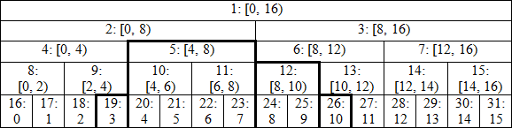
\includegraphics{pictures/segtree.png}

Реализация будет такой --- сделаем рекурсивную функцию $get$, которая хочет обойти дерево, зайти во все <<ключевые>> отрезки запроса, и посчитать итоговый ответ. Для $get(v,\,l,\,r)$ бывает три случая:
\begin{itemize}
\item $v$ не отвечает ни за что из отрезка $[l,\,r]$, поэтому не делаем ничего и прекращаем работу.
\item $[l,\,r]$ содержит отрезок вершины $v$, и тогда можно обработать этот отрезок и прекратить работу.
\item Иначе надо спуститься в детей, и повторить процесс
\end{itemize}

\paragraph{Lazy propagation.} Пусть у нас появился запрос $change$, модифицирующий отрезок. Будем хранить в вершине пометки вида <<мы хотели сделать со всеми детьми такую-то операцию изменения>>, которые мы изначально будем проставлять с запросом изменения на все <<ключевые отрезки>>. При этом во время запроса изменения мы по сути не сделаем изменений, только проставим пометки. Но теперь мы при каждом обращении к вершине проталкиваем модификатор (если есть) вниз, и меняем текущее значение $value$. Таким образом, после проталкивания все величины остаются валидными (кроме тех, которые находятся где-то глубоко в дереве, но к которым мы не спустились). 

\textit{Иначе говоря, мы считаем, что перед тем, как обратиться к какой-то вершине, мы обязаны обратиться ко всем вершинам-предкам, и тогда можем гарантировать, что в ней будут храниться актуальные значения параметров.}

Требования к lazy propagation~--- дистрибутивность операции $change$ относительно $\oplus$, а также модификаторы также должны являться полугруппой.


\end{document}
